% !TEX root = TeX/Raman.tex

\begin{center}
    \begin{huge}
    \textbf{S3:\\}
    \vspace{0.5cm}
    \textbf{Raman-Mikroskopie-Versuch}
    \end{huge}
    \vspace{0.5cm}
\end{center}
\section{Molekül und Festkörperschwingungen}\label{sec:vib}
Die Schwingungsspektroskopie beschäftigt sich mit der Anregung von Molekül- und Festkörperschwingungen. 
Im Spektrum zeigen sich diese Schwingungen als bestimmte Linien oder Banden bei charakteristischen Energien. 
Die genaue energetische Lage dieser Banden kann relativ einfach aus den Bindungseigenschaften der Moleküle oder Kristalle abgeschätzt werden.
Hierbei kann die Bindung zwischen zwei Atomen als eine Art Feder betrachtet werden. Aus der klassischen Mechanik folgt, dass die 
Schwingungsfrequenz einer solchen Feder-Schwingung von der Federkonstante $k$ und der reduzierten Masse $\mu$ der beiden Atome abhängt.
\begin{equation}
    \omega = \sqrt{\frac{k}{\mu}} 
    \label{eq:schwingungsfrequenz}
\end{equation}
Mit:
\begin{itemize}
    \item $k$: Kraftkonstante der Bindung [N/m]
    \item $\mu$: reduzierte Masse der beiden Atome [kg]
\end{itemize}

Stark gebundene und leichte Atome (großes $k$, kleine $\mu$) führen somit zu hohen Schwingungsfrequenzen, während schwach gebundene oder schwere Paare tiefere Frequenzen aufweisen. 

\begin{figure}[H]
    \centering
    
\includegraphics[width=0.4\textwidth]{1_Skript/Inkscape/Feder.png}
    \caption{Vorstellung einer Bindung als Feder. Die Schwingungsfrequenz hängt von der Kraftkonstante $k$ und der reduzierten Masse $\mu$ ab.}
    \label{fig:Feder}
\end{figure}

Dieses Modell erlaubt eine erste Abschätzung der Position von Schwingungsbanden im IR- oder Raman-Spektrum aus den Kraftkonstanten und Massen der Bindungspartner. In realen Molekülen weichen 
die Schwingungsenergien durch Anharmonizität leicht von der harmonischen Näherung ab, aber Gleichung \ref{eq:schwingungsfrequenz} bietet trotzdem eine wichtige Grundlage für das Verständnis von Schwingungsspektren.\\
In Festkörpern reicht es nicht mehr aus, nur die Schwingungen einzelner Atome oder Moleküle zu betrachten. Stattdessen bewegen sich hier viele Atome gemeinsam. 
Diese kollektiven Festkörperschwingungen durchziehen das gesamte Kristallgitter und werden als Phononen bezeichnet.

\begin{figure}[H]
    \centering
    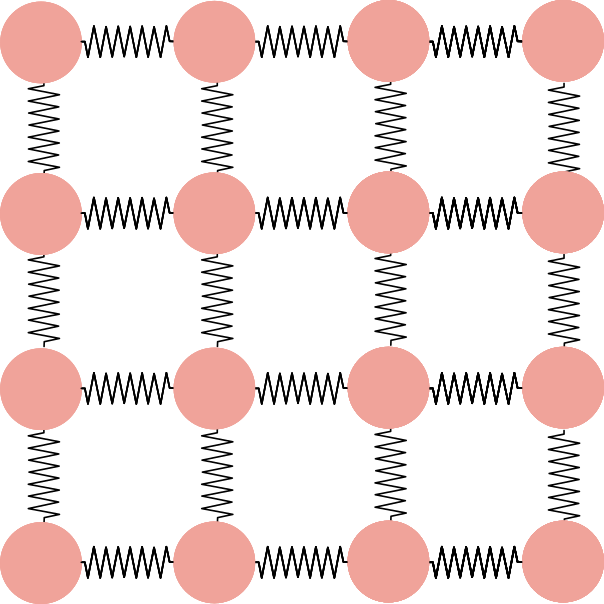
\includegraphics[width=0.4\textwidth]{1_Skript/Inkscape/phonon.png}
    \caption{Festkörperschwingungen werden als Phononen bezeichnet. Sie sind kollektive Schwingungen des gesamten Kristallgitters. Alle Atome in einem Gitter sind durch Bindungen mit einer Federkonstante verbunden.}
    \label{fig:Phonon}
\end{figure}

\section{Raman-Effekt}\label{sec:raman}
Beim Raman-Effekt handelt es sich um einen sogenannten Streuprozess. Das heißt, ein Photon trifft auf ein Molekül oder einen Festkörper, regt 
dabei das System kurzzeitig in einen virtuellen Zustand, und direkt danach folgt die Abgabe eines gestreuten Photons. Dieser virtuelle Zustand 
ist kein \glqq{}echter\grqq{} angeregter Zustand, wie er zum Beispiel bei der Fluoreszenz auftritt. Er hat also keine definierte Lebensdauer 
im Sinne einer messbaren Aufenthaltszeit, sondern entsteht und zerfällt praktisch sofort, die Lebensdauer des angeregten virtuellen Zustand 
liegt somit im Bereich von weniger als 1~fs.\\
Wird die Raman-Streuung mit der IR-Spektroskopie verglichen, so unterscheidet sich der Raman-Effekt von der IR-Absorption in wesentlichen Punkten.
Zum einen ist die Raman-Streuung ein nicht resonanter Prozess, das heißt, die Energie des einfallenden Lichts entspricht nicht zwangsläufig der Energiedifferenz zwischen 
zwei Zuständen unseres Systems. Der Raman-Effekt wird demnach unabhängig von der Wellenlänge des einfallenden Lichts beobachtet.
Zum anderen bedingt der Raman-Effekt eine Änderung der Polarisierbarkeit des Moleküls während der Schwingung, während für
die IR-Aktivität eine Änderung des Dipolmoments während der Schwingung notwendig ist. Die Polarisierbarkeit $\alpha$ beschreibt, 
wie leicht sich die Elektronenhülle eines Moleküls/ Festkörpers durch ein elektrisches Feld verformen lässt.
Man kann diese auch als Proportionalität zwischen einer induzierten Polarisation $\vec{P}_{ind}$ und dem anregenden elektrischen Feld $\vec{E}$ verstehen:
Die Polarisierbarkeit ist demnach ein dreidimensionales Konstrukt und kann als Tensor aufgefasst werden:

\begin{equation}
    \vec{P}_{ind} = \alpha \cdot \vec{E}
\end{equation}
Mit:
\begin{itemize}
    \item $\vec{P}_{ind}$: Induzierte Polarisation [C/m$^2$]
    \item $\alpha$: Polarisierbarkeitstensor [C/V$\cdot$m]
    \item $\vec{E}$: Anregendes elektrisches Feld [V/m]
\end{itemize}

Schwingungen, die die Polarisierbarkeit $\alpha$ ändern, sind 
Raman-aktiv, während solche mit Dipolmomentänderung IR-aktiv sind, dadurch ergänzen sich IR- und Raman-Spektroskopie häufig.\\

\begin{figure}[H]
    \centering
    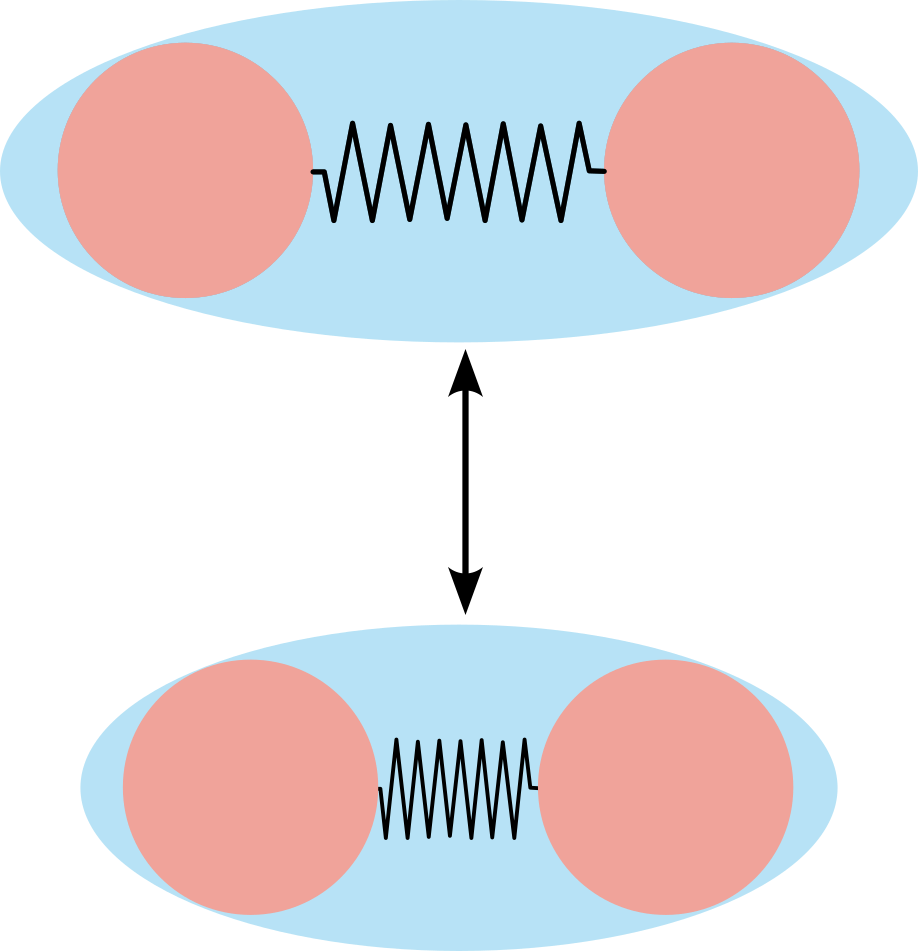
\includegraphics[width=0.5\textwidth]{1_Skript/Inkscape/Polarisierbarkeit.png}
    \caption{Schematische Darstellung der Polarisierbarkeit eines Moleküls. Die Polarisierbarkeit  in blau  ändert sich während der Schwingung, was für die Raman-Streuung notwendig ist.}
    \label{fig:Polarisierbarkeit}
\end{figure}

Wird jedoch Materie mit Licht bestrahlt, so wird das Licht nur zu einem geringen Teil inelastisch gestreut. Der Großteil des Lichts wird elastisch gestreut, was als Rayleigh-Streuung bezeichnet wird.
Nur jedes tausendste bis zehntausendste Photon wird inelastisch gestreut.\\
Sowohl die IR- als auch die Raman-Spektroskopie zählen zu den Verfahren der linearen Spektroskopie.
Das bedeutet: Für jedes eingestrahlte Photon wird maximal ein Photon absorbiert oder gestreut, das System reagiert also proportional zur einfallenden Lichtintensität. Dies ist für 
Auswertung und Interpretation der Spektren von besonderer Bedeutung, da demnach das detektierte Signal eine Summe aller Effekte ist. Wodurch die Zusammensetzung des untersuchten Systems 
rekonstruiert wetden kann.\\

Das detektierte Raman-Streusignal hat dann die Energie des einfalenden Lichts ($\tilde{\nu}_0)$ plus oder minus der Energieänderung, die durch die Schwingung 
des Moleküls beziehungsweise Festkörpers ($\tilde{\nu}_v)$ verursacht wird.
Ist das detektierte Photon energieärmer so wir dieser Effekt als Stokes-Raman bezeichnet, während der seltener auftretende energieerhöhter Anteil als Anti-Stokes-Raman bezeichnet wird.
\begin{eqnarray}
    \tilde{\nu}_{Stokes} = \tilde{\nu}_0 - \tilde{\nu}_v 
    \label{eq:stokes} \\
    \tilde{\nu}_{Anti-Stokes} = \tilde{\nu}_0 + \tilde{\nu}_v
    \label{eq:anti-stokes}  
\end{eqnarray}

\begin{figure}[H]
    \centering
    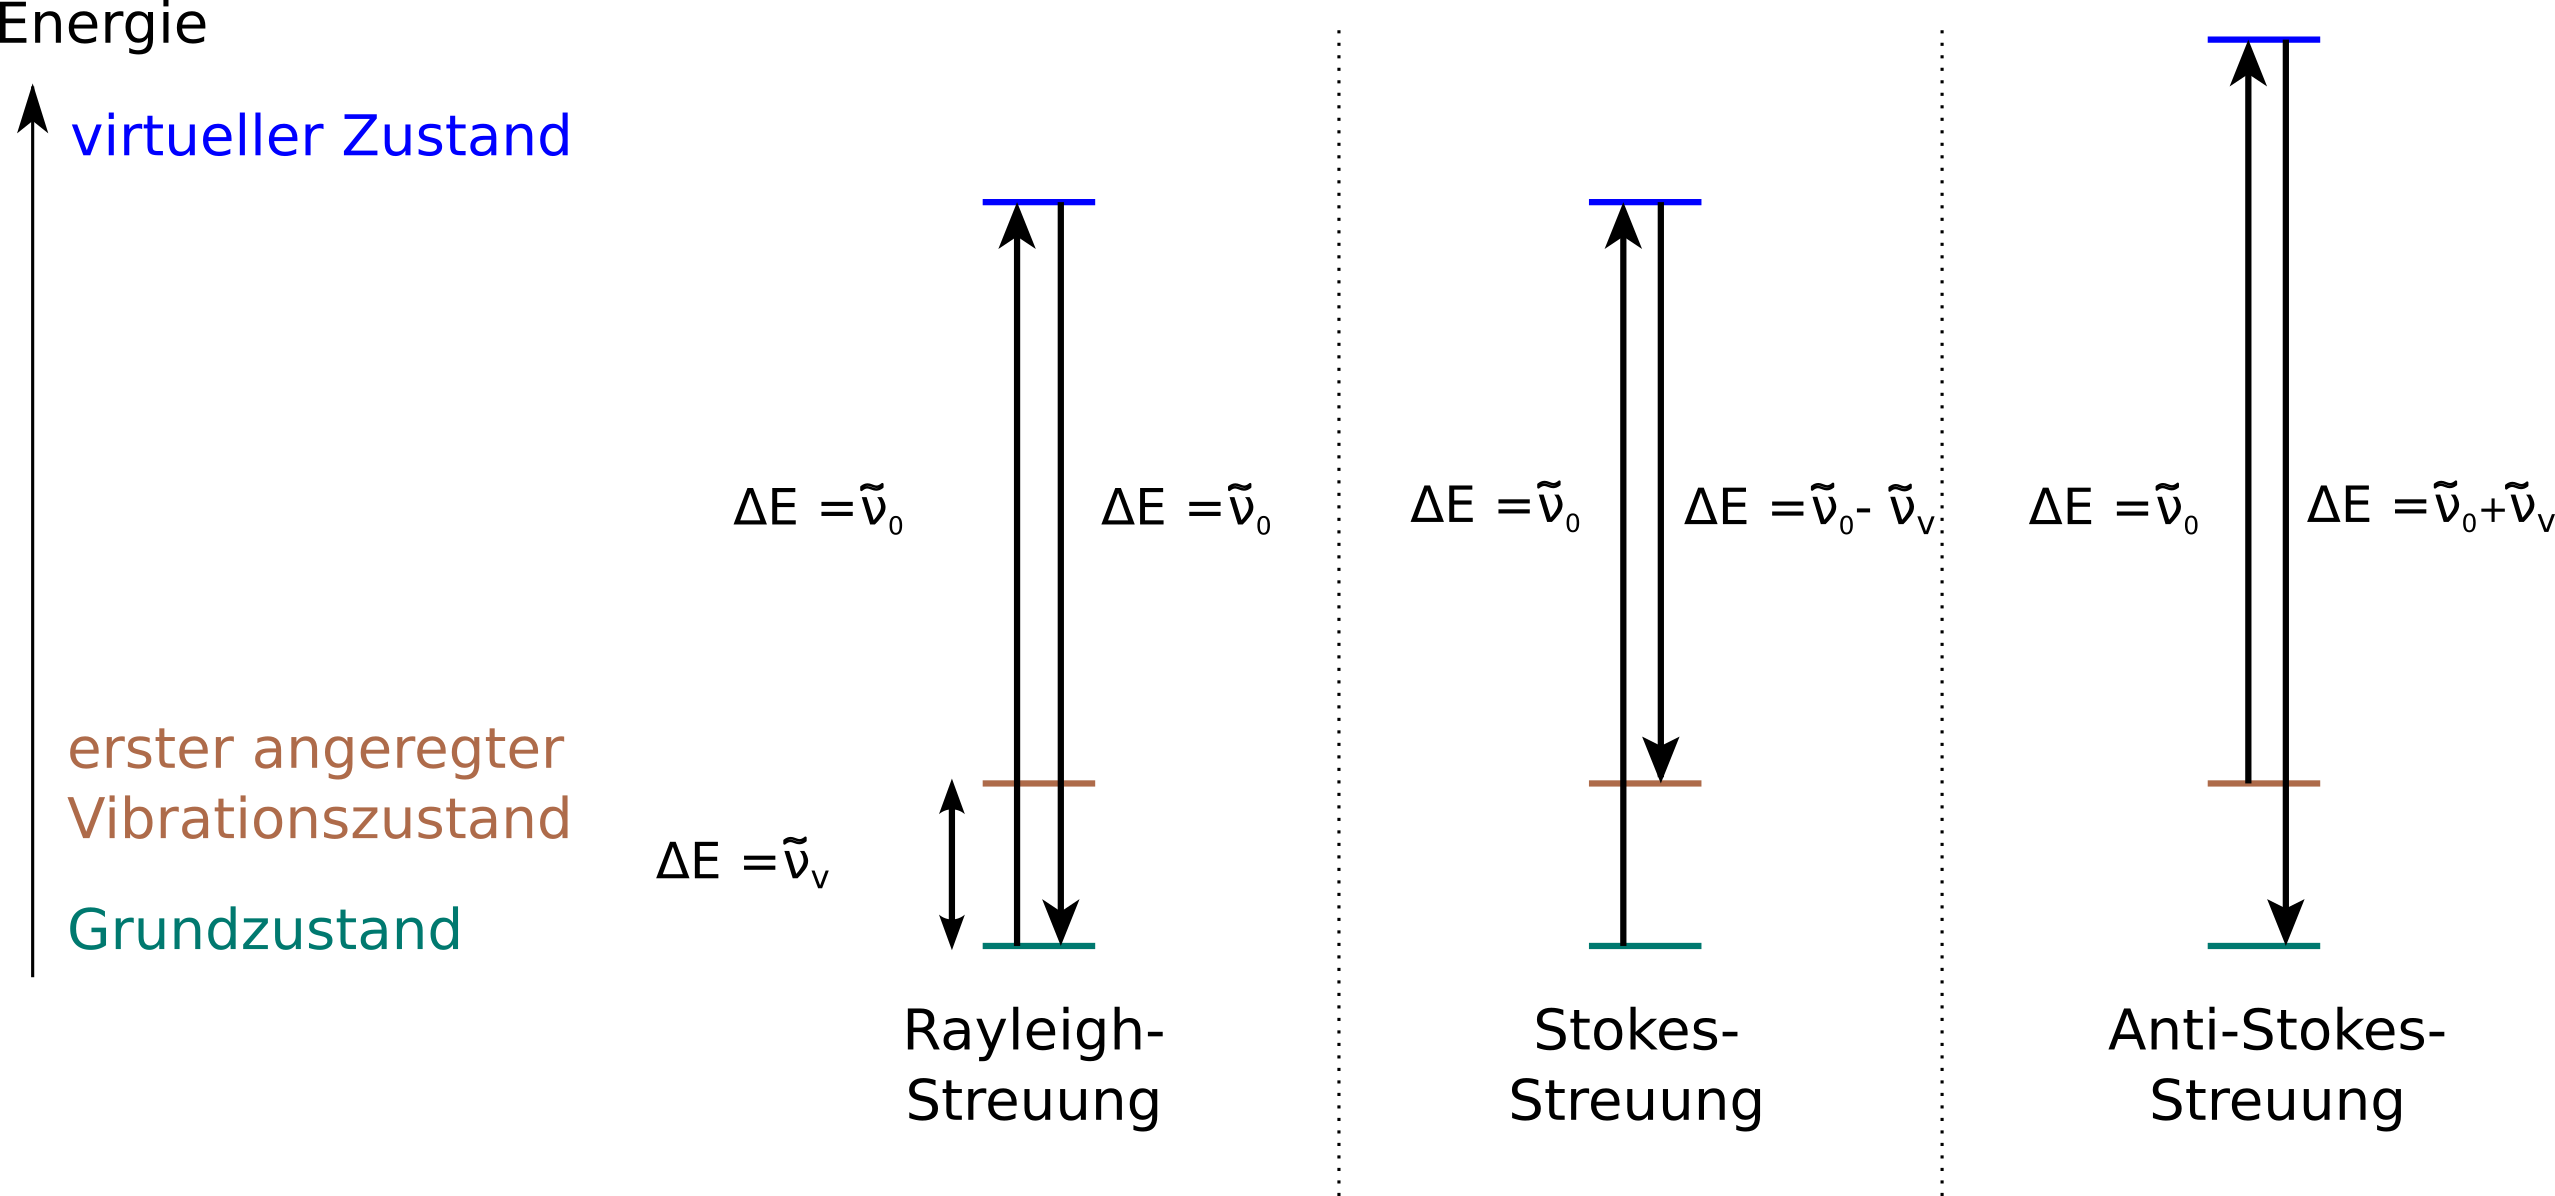
\includegraphics[width=0.8\textwidth]{1_Skript/Inkscape/Raman.png}
    \caption{Schematische Darstellung des Raman-Effekts. Ein Photon trifft auf ein Molekül, regt es in einen virtuellen Zustand an und wird dann mit einer Frequenzänderung gestreut.}
    \label{fig:Raman}
\end{figure}


Die relativen Anteile der Stokes- und Anti-Stokes-Banden sind direkt von der Besetzung der beteiligten Schwingungszustände und demnach von der Boltzmannverteilung abhängig.

\begin{equation}
    \frac{I_{Anti-Stokes}}{I_{Stokes}} = \frac{N_1}{N_0} = \text{exp}\left(-\frac{\tilde{\nu}_v}{kT}\right)
\end{equation}

Demnach ergibt sich bei Raumtemperatur für eine typische Schwingungsfrequenz von etwa 1000~cm$^{-1}$ ein Intensitätsverhältnis von etwa 1:100 zwischen Stokes- und Anti-Stokes-Banden.\\
Diese unterscheid sich grundlegend von der IR-Absorption, bei der die Energie des einfallenden Lichts genau der Energiedifferenz zwischen dem Grundzustand und dem angeregten Zustand des Moleküls entspricht.

Jede beobachtbare Bande ob in IR- oder Raman-Spektren lässt sich mindestens durch drei Parameter charakterisieren: eine Energie (meist in cm$^{-1}$ angegeben), 
die Intensität und die spektrale Breite der Bande. Die Energie entspricht dabei der Schwingungsenergie, die Intensität liefert Informationen über die Raman-Aktivität und die Anzahl der Oszillatoren, 
während die Halbwertsbreite (engl. \textit{full width at half maximum}, FWHM) Rückschlüsse auf die Lebensdauer des Schwingungszustands oder auf Störungen im Festkörper geben kann. 
Die Halbwertsbreite einer solchen Schwingungsbande, sowohl im IR- als auch im Raman-Spektrum, wird im Prinzip durch die Lebensdauer ($\tau$) des angeregten Schwingungszustands begrenzt:
\begin{equation}
    \Delta\tilde{\nu} = \frac{1}{2\pi c\tau}
\end{equation}
Mit:
\begin{itemize}
    \item $\Delta\tilde{\nu}$: Halbwertsbreite der Bande [cm$^{-1}$]
    \item $c$: Lichtgeschwindigkeit [m/s]
    \item $\tau$: Lebensdauer des angeregten Schwingungszustands [s]
\end{itemize}
Die Halbwertsbreite ist also umgekehrt proportional zur Lebensdauer des angeregten Schwingungszustands. Je kürzer die Lebensdauer, desto breiter die Bande. Dies 
ist eine direkte Folge der Energie-Zeit-Unschärferelation:
\begin{equation}
    \Delta E \cdot \Delta t \geq \frac{\hbar}{2}
\end{equation}
Mit:
\begin{itemize}
    \item $\Delta E$: Energieunschärfe [J]
    \item $\Delta t$: Zeitunschärfe [s]
    \item $\hbar$: reduzierte Planck-Konstante ($\hbar = h/2\pi$) [J$\cdot$s]
\end{itemize}

Typische Lebensdauern von Schwingungszuständen liegen im Bereich von 10$^{-12}$-10$^{-14}$ Sekunden, was zu Halbwertsbreiten im Bereich von 1-10 cm$^{-1}$ führt.\\
In der Praxis wird eine solche Bande häufig durch eine Lorentzfunktion beschrieben.

\begin{equation}
    I(\tilde{\nu}) = \frac{I_0}{1 + \left(\frac{\tilde{\nu} - \tilde{\nu}_0}{\Gamma/2}\right)^2}
\end{equation}
Mit:
\begin{itemize}
    \item $I(\tilde{\nu})$: Intensität bei der Wellenzahl $\tilde{\nu}$ [a.u.]
    \item $I_0$: Maximale Intensität der Bande [a.u.]
    \item $\tilde{\nu}_0$: Bandenposition  [cm$^{-1}$]
    \item $\Gamma$: Halbwertsbreite [cm$^{-1}$]
\end{itemize}

In komplexeren Fällen können auch Profile mit mehr als drei Parametern wie z.B. Voigt-Profile verwendet werden, welche aber an dieser Stelle nicht weiter behandelt werden sollen.


\subsection{Raman-Spektren von Metallen und Metalloxiden}

Metalle und Metalloxide zeigen im Raman-Verhalten deutliche Unterschiede. Für das Auftreten von Raman-Banden muss sich, wie zuvor erwähnt, die Polarisierbarkeit während einer Schwingung ändern
Reine Metalle besitzen in der Regel keine Raman-aktiven Gittermoden. Da einerseits in einem monatomaren Kristall keine optischen Phononen existieren und andererseits die frei beweglichen 
Leitungselektronen die elektromagnetische Anregung stark abschirmen.
Viele Metalle zeigen daher keine ausgeprägten Raman-Banden. Metalloxide hingegen bestehen aus verschiedenen Atomarten pro Einheitszelle und haben polare Bindungen. Ihre Gitter besitzen demnach 
optische Phononen, die Raman-aktiv sein können. Infolgedessen liefern Metalloxide (z.B. \ce{TiO2}, \ce{Fe2O3}, \ce{MgO} etc.) meist intensive Raman-Spektren mit 
charakteristischen Banden im Bereich von 200-800~cm$^-1$ auf, während bei reinen Metallen oft nur ein Untergrund, welcher auf die thermische Anregung durch den Laser zurückzuführen ist, beobachtbar sind.
\clearpage
\section{Auswertung von Raman-Spektren}\label{sec:analysis}
Ein experimentell aufgenommenes Raman-Spektrum setzt sich meist aus mehreren Beiträgen zusammen. Idealerweise werden Raman-Banden bei den charakteristischen Verschiebungen beobachtet, die 
dem untersuchten Material entsprechen. In der Praxis liegen diese Banden jedoch häufig auf einer Basislinie bzw. einem breiten Hintergrund, der verschiedene Ursachen haben kann. Sowohl 
der Messaufbau als auch die Probe selbst können Hintergrundsignale verursachen. Insbesondere können hohe Laserintensitäten zu einer lokalen Erwärmung der Probe führen, was eine starke, 
breitbandige Schwarzkörper-Emission oder auch eine  Fluoreszenz hervorrufen kann. Diese beiden Effekte können einen breiten und intensiven Hintergrund erzeugen, der das eigentliche 
Raman-Signal überlagert und unter Umständen sogar vollständig verdecken kann. Alle Effekte überlagern sich additiv, sodass die eigentlichen Raman-
Banden nicht immer eindeutig erkannt werden können.\\
In der Literatur wird einer Bande im Spektrum häufig eine einzelne Molekülschwingung zugeordnet. Tatsächlich handelt es sich jedoch meist um eine Überlagerung vieler verschiedener
molekularer Bewegungen. Daher ist es wenig sinnvoll, das Auftreten einzelner Banden als eindeutige Identifikatoren für bestimmte Systeme heranzuziehen. Stattdessen sollte das 
Gesamtspektrum mit allen Banden und ihren relativen Intensitäten als Referenz für ein System betrachtet werden. Ein gemessenes Raman-Spektrum $S(\tilde{\nu})$ lässt sich daher 
konzeptionell als Linearkombination der Signalbeiträge verschiedener Schwingungsmoden auffassen:

\begin{equation}
    S(\tilde{\nu}) = R(\tilde{\nu}) + B(\tilde{\nu}) + U(\tilde{\nu})
\end{equation}
Mit:
\begin{itemize}
    \item $S(\tilde{\nu})$: gemessenes Raman-Spektrum 
    \item $R(\tilde{\nu})$: reines Raman-Streusignal 
    \item $B(\tilde{\nu})$: Basislinie 
    \item $U(\tilde{\nu})$: unspezifischer Hintergrund 
\end{itemize}

Demnach ist für eine erfolgreiche Auswertung eine Analyseprozedur notwendig, welche im Folgenden beschrieben wird.

\subsection{Analyseprozedur eines Raman-Spektrums}

Die Auswertung experimenteller Raman-Spektren erfolgt in mehreren aufeinanderfolgenden Schritten, um verlässliche und vergleichbare spektrale Informationen zu erhalten.

\begin{enumerate}
    \item \textbf{Kalibrierung}
    \begin{itemize}
        \item Überprüfung der Wellenzahlkalibrierung des Spektrometers.
        \item Kalibrierung erfolgt in der Regel mit bekannten Referenzmaterialien, z.B. Silizium (\ce{Si})
    \end{itemize}
    \item \textbf{Entfernen von Störsignalen}
        \begin{itemize}
        \item Aufgrund von kosmischer Strahlung kann es zu sogenannten Artefakten kommen. Diese sind in der Regel als 
        Peaks, die deutlich unter der FWHM von Raman-Banden liegen (1-10~cm$^{-1}$), zu erkennen. Meist sind diese nur
         einzelne Pixel breit und können durch eine einfache Interpolation entfernt werden.
        \item Werden Artefakte vermutet, welche breiter als einzelne Pixel sind. So ist hier Vorsicht geboten. Eine einfache Interpolation
        kann zu einer Verfälschung der Daten führen. Die Identifikation von breiten Artefakten kann nur durch den Vergleich 
        mit Referenzen erfolgen. Aus diesem Grund sollte immer für eine Erhöhung des Signal-Rausch-Verhältnisses eher die Spektrenanzahl 
        erhöht werden, als die Messzeit zu verlängern.
    \end{itemize}
    \item \textbf{Normierung}
    \begin{itemize}
        \item Anpassung der Intensität, um spektrenübergreifende Vergleichbarkeit zu ermöglichen.
        \item Methoden: Normierung auf die maximale Peak-Intensität. Alle Intensitäten werden durch die Intensität des stärksten Peaks geteilt, sodass dieser auf 1 normiert wird.
        \item Alternativ: Normierung auf einen bestimmten Referenzpeak.
    \end{itemize}
    \item \textbf{Quantitative Datenanalyse}
    \begin{itemize}
        \item Anwendung statistischer Methoden wie Hauptkomponentenanalyse (engl. \textit{Principal Component Analysis},PCA) zur Extraktion von Mustern aus komplexen Datensätzen.
        \item Nutzung von Methoden wie Partial Least Squares (PLS) für quantitative Korrelationen zwischen Spektraldaten und Probenparametern.
    \end{itemize}
        \item \textbf{Optional: Peak-Identifikation und -Quantifizierung}
    \begin{itemize}
        \item Identifikation relevanter Raman-Banden.
        \item Analyse dieser durch Kurvenanpassung mit Lorentz-Funktionen zur Bestimmung von Peak-Position, Höhe und Halbwertsbreite.
    \end{itemize}
    
\end{enumerate}

Jeder dieser Schritte kann je nach Messung und Material spezifisch angepasst werden. Die sorgfältige Durchführung der beschriebenen Schritte ist entscheidend für 
eine verlässliche und reproduzierbare Raman-Analyse.

\section{Experimentelle Aspekte}\label{sec:experiment}
Das in diesem Versuch verwendete Raman-Mikroskop der Firma \textit{Lightnovo} kombiniert einen Raman-Spektrometeraufbau mit einem optischen Mikroskop.
Die wichtigsten technischen Parameter und Messbedingungen des Raman-Mikroskops sind in Tabelle~\ref{tab:785nm-parameter} zusammengefasst:

\begin{table}[H]
    \centering
    \caption{Technische Parameter des RG-HR-Raman-Mikroskops der Firma \textit{Lightnovo}}
    \begin{tabular}{l|l}
        \textbf{Parameter}                & \textbf{Wert}        \\
        \hline
        Laserwellenlänge                  & 785~nm                        \\
        Leistungsbereich auf Probe        & 0.1--65~mW                  \\
        Spektralbereich                   & 450--1800~cm$^{-1}$       \\
        Spektrale Auflösung               & 1.5--3~cm$^{-1}$        \\
        Laterale  Auflösung  (xy)         & 600~nm                        \\
        Axiale Auflösung (z)              & 1500~nm                       \\
        Mikroskopiemodus                  & Rückstreuung            \\
        Maximaler Verfahrweg              & 102x102x25~mm$^3$ \\
        Lateraler Schritt                 & 100~nm                        \\
        Axialer Schritt                   & 100~nm        \\
        \hline                
    \end{tabular}
    \label{tab:785nm-parameter}
\end{table}

\clearpage
\section{Literatur}
Die in diesem Versuch behandelten Themenkreise finden sich in der folgenden Literatur ausführlich dargestellt:
\begin{enumerate}
    \item B. Schrader, Infrared and Raman-Spectroscopy, Verlag Chemie, Weinheim, 1980, Kap. 2
    \item G. Herzberg, Molecular Spectra and Molecular Structure, Vol. II, Infrared and Raman Spectra of Polyatomic Molecules, Krieger 1991.
    \item F. Engelke, Aufbau der Moleküle, Teubner 1992
    \item Barton B, Thomson J, Lozano Diz E, Portela R. Chemometrics for Raman Spectroscopy Harmonization. Applied Spectroscopy. 2022;76(9):1021-1041.\\
    \texttt{DOI:}\href{https://www.doi.org/10.1177/00037028221094070}{10.1177/00037028221094070}
    \item \href{https://de.wikipedia.org/wiki/Raman-Streuung}{Wikipedia: Raman-Streuung} Aufgerufen am 03.06.2025
    \item \href{https://www.spectroscopyonline.com/view/lineshapes-ir-and-raman-spectroscopy-primer}{Lineshapes in IR- and Raman-Spectroscopy: A Primer} Aufgerufen am 03.06.2025
\end{enumerate}